\documentclass[11pt,a4paper]{article}

\usepackage[margin=25mm]{geometry}
\usepackage{amsmath,amssymb}
\usepackage{graphicx}
\usepackage{natbib}
\usepackage[hidelinks]{hyperref}

\graphicspath{{figures/}}

\newcommand{\Bo}{\mathcal{B}o}
\newcommand{\Rb}{R_b}
\newcommand{\Rc}{R_c}
\newcommand{\Rzero}{R_0}

\title{Young--Laplace initial conditions for bursting-bubble simulations}
\author{Vatsal Sanjay\\[0.4em]
\small CoMPhy Lab, Department of Engineering, Durham University}
\date{August 2026}

\begin{document}
\maketitle

\begin{abstract}
A bursting-bubble computation starts from an open cavity at a free surface.
That cavity is the Young--Laplace equilibrium of a prescribed gas volume.
The Bond number based on the equivalent-sphere radius sets how far gravity
pulls the bubble away from a sphere. We document the Python generator that
builds these shapes for Basilisk Stage~1. Bond continuation from a cheap
spherical seed replaces the old one-shot curvature guess. At vanishing Bond
the meniscus match is undefined, so the generator writes a unit sphere
meeting a plane, regularized by a fillet of scale~$\delta$. The opening
angle recovers the comparison of \citet{Lhuissier2012}, and the written
polyline sits on the repository's shipped $\Bo=10^{-3}$ file.
\end{abstract}

\section{Introduction}
\label{sec:intro}

When a bursting-bubble computation starts, the thin film that closed the
cavity has already gone. The remaining geometry is an open cavity meeting a
free surface. That shape is not a drawing choice. It is the quasi-static
Young--Laplace equilibrium of a gas volume at a liquid--air interface
\citep{Princen1963}, and it sets the first capillary waves that later focus
at the bottom of the cavity.

The Bond number
\begin{equation}
  \Bo = \frac{\rho g \Rzero^2}{\gamma}
\end{equation}
compares gravity to surface tension on the equivalent-sphere radius
$\Rzero$, the radius of the sphere with the same gas volume. Lengths in
this report, and in the Basilisk solvers, are scaled by $\Rzero$. That
choice is not the same as a Bond number based on the bottom curvature
radius. At small Bond the cavity is nearly spherical. As Bond increases the
bubble flattens, the submerged profile lengthens, and the opening left by
the ruptured film widens. \citet{Lhuissier2012} mapped that opening against
the capillary length. Direct numerical studies of bursting, including our
viscoplastic calculations \citep{Sanjay2021} and the Newtonian
cross-validation of \citet{Deike2018}, have typically taken a
near-spherical cavity at $\Bo=10^{-3}$ rather than solving the equilibrium
at the Bond number of the run.

The MATLAB driver \texttt{InitialCondition.m} that accompanies
\citet{Lhuissier2012} already solves this nested shooting problem. Working
copies of that driver each carried a different first guess for the bottom
curvature. A cold start at large Bond with a guessed $\Rb^{\mathrm{max}}$
is fragile. The Python generator in
\texttt{simulationCases/initialConditions/} ports that construction, walks
Bond upward from $10^{-3}$, and writes the polyline that Stage~1 of the
Basilisk bursting-bubble solvers \citep{Popinet2009} consumes. At strictly
vanishing Bond the $2/\Bo$ meniscus match is undefined. That limit is a
unit sphere meeting a plane, regularized by a fillet of scale~$\delta$.

The report is organized as follows.
\S\ref{sec:problem} states the equilibrium problem.
\S\ref{sec:shoot} describes the nested shoot and the continuation.
\S\ref{sec:fillet} treats the neck fillet.
\S\ref{sec:zero} is the Bond-zero geometry.
\S\ref{sec:checks} records the file convention and the checks against
\citet{Lhuissier2012}.
\S\ref{sec:cli} is the command line.
We close with the limitations of a quasi-static initial cavity.

\section{Equilibrium problem}
\label{sec:problem}

The generating curve is axisymmetric. The tangent angle $\varphi$ is
measured from the horizontal, starting at the south pole
($\varphi=0$) and running toward the top ($\varphi=\pi$). Three pieces
meet at a contact station $\varphi_c$.

The submerged cavity $(\mathcal{R}(\varphi),\mathcal{Z}(\varphi))$
satisfies the Young--Laplace balance written as an ODE in $\varphi$,
\begin{align}
  \frac{\mathrm{d}\mathcal{R}}{\mathrm{d}\varphi}
  &=
  \frac{\mathcal{R}\cos\varphi}{\mathcal{R}\,(2/\Rb + \Bo\,\mathcal{Z})-\sin\varphi},
  \label{eq:dR}
  \\
  \frac{\mathrm{d}\mathcal{Z}}{\mathrm{d}\varphi}
  &=
  \frac{\mathcal{R}\sin\varphi}{\mathcal{R}\,(2/\Rb + \Bo\,\mathcal{Z})-\sin\varphi}.
  \label{eq:dZ}
\end{align}
The south pole is regularized by a small start $\varphi_0=10^{-5}$ with
$(\mathcal{R},\mathcal{Z})=(\Rb\sin\varphi_0,\,\Rb(1-\cos\varphi_0))$.
The bottom curvature radius $\Rb$ is unknown. We use the
$\sin\varphi$ form of \eqref{eq:dZ} rather than
$\tan\varphi\,\mathrm{d}\mathcal{R}/\mathrm{d}\varphi$, so the equator
stays regular.

A spherical cap of radius $\Rc$ matches slope and curvature at the
contact. The far-field free surface is an outer meniscus that must
approach a constant height $h_\infty$ as $\mathcal{R}\to\infty$. Pressure
balance between the south pole, the cap, and that far field fixes
\begin{equation}
  h_\infty = \frac{2}{\Bo}\left(\frac{2}{\Rc}-\frac{1}{\Rb}\right).
  \label{eq:hinf}
\end{equation}
The enclosed gas volume, scaled by $4\pi/3$, is
\begin{equation}
  \frac{3}{4}\int \mathcal{R}^2\,\mathrm{d}\mathcal{Z} = 1,
  \label{eq:vol}
\end{equation}
with the integral taken over the submerged profile and the spherical cap.

The opening angle of \citet{Lhuissier2012} is
$\alpha_c=\pi-\varphi_c$. Their small-Bond estimate, when
$\Rc\sim\Rzero$, is
\begin{equation}
  \alpha_c = \frac{1}{2\sqrt{3}}\,\frac{\Rc}{a},
  \qquad
  a = \sqrt{\gamma/\rho g} = \Rzero/\sqrt{\Bo}.
  \label{eq:alpha}
\end{equation}
Figure~\ref{fig:geometry} shows one hit at $\Bo=1$ in the integration
coordinates, together with the family of written Basilisk polylines.

\begin{figure}
  \centering
  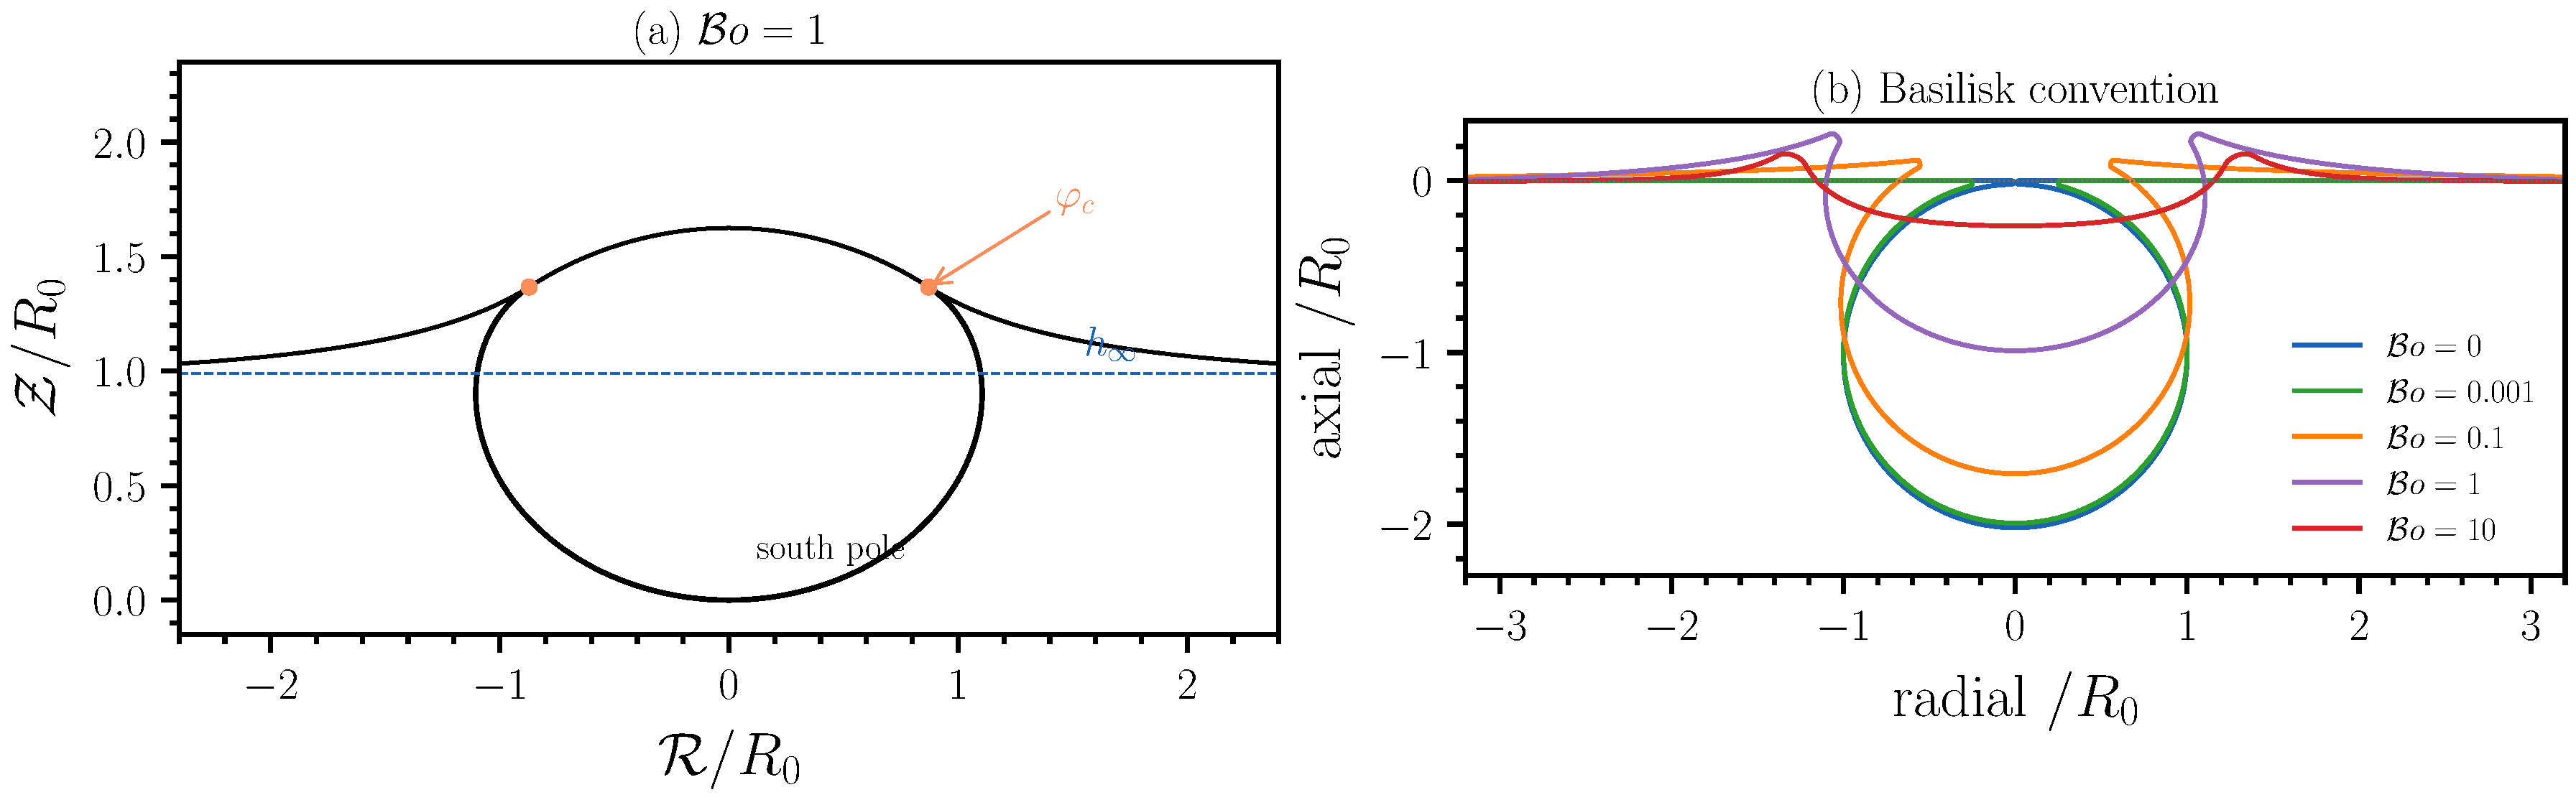
\includegraphics[width=0.92\textwidth]{geometry.pdf}
  \caption{Equilibrium construction.
    (a)~Submerged cavity, spherical cap, and outer meniscus at
    $\Bo=1$, plotted with $\mathcal{Z}$ upward from the south pole.
    The contact station is $\varphi_c$; the opening is
    $\alpha_c=\pi-\varphi_c$.
    (b)~The same generator written in the Basilisk convention, cavity in
    $-\mathrm{axial}$, free surface at $\mathrm{axial}=0$, for
    $\Bo=0$, $10^{-3}$, $0.1$, $1$, and $10$. The $\Bo=0$ curve is the
    sphere--plane construction of \S\ref{sec:zero}.}
  \label{fig:geometry}
\end{figure}

\section{Nested shooting and Bond continuation}
\label{sec:shoot}

Two unknowns remain, $\Rb$ and $\varphi_c$. The outer loop shoots
$\Rb$ so that \eqref{eq:vol} holds. For each trial $\Rb$ the inner loop
shoots $\varphi_c$ so that the meniscus meets $h_\infty$.

The meniscus residual is not $Z(R_{\max})-h_\infty$. Beyond a few
capillary lengths the decaying meniscus mode is swamped by the growing
one, and that far-field difference jumps discontinuously with
$\varphi_c$. We match at
$\mathcal{R}_c + O(1/\sqrt{\Bo})$, a station a few capillary lengths
out from the contact. The MATLAB driver integrated to a fixed
$\texttt{TailxMax}$ of $8$ (sometimes $4$) and only afterwards padded
the free surface to $32$. Checking at infinity is neither necessary
nor stable.

Linear interpolation of $(\mathcal{R},\mathcal{Z})$ onto $\varphi_c$
uses the local interval $\varphi_{i+1}-\varphi_i$. The MATLAB driver
used a broken denominator here. That bug is silent at small Bond, where
$\varphi_c$ sits near $\pi$ and the samples are dense. It is not silent
once the contact walks down the profile.

A volume residual that does not change sign is not reported as a root.
The $\Rb$ bracket expands, first from a previous hit if one exists, and
otherwise from a Bond-dependent upper bound. Failures return an error
rather than a guessed polyline.

Continuation replaces the old per-Bond $\Rb$ guesses. Small-Bond shapes
are nearly spherical ($\Rb\approx 1$). Walking $\Bo$ upward, using each
accepted $(\Rb,\varphi_c)$ as the next guess, is much more stable than a
cold start at large Bond. The ladder starts at $10^{-3}$ and grows by a
ratio of at most $2$ until the target. A comma-separated Bond list
continues from the previous requested value. A prior shape is reused
only when its Bond is at or below the target. Reusing a higher-Bond hit
for a lower target writes the wrong geometry into
\texttt{Bo\%5.4f.dat}.

The Young--Laplace shooter refuses $\Bo\le 0$ and
$\Bo<10^{-6}$. Those limits belong to \S\ref{sec:zero}.

\section{Neck fillet}
\label{sec:fillet}

Removing the film leaves a curvature singularity where the cavity meets
the free surface. Stage~1 cannot ingest that corner. The MATLAB driver
inserted a circular fillet whose radius can change sign with the sample
index. We replace that construction with a $C^1$ cubic Hermite blend on
the contact-truncated profiles $(\mathcal{R}_{\mathrm{sub}},
\mathcal{Z}_{\mathrm{sub}}, \varphi_{\mathrm{sub}})$ and the nearby
meniscus. Position and tangent are matched at both cuts. The default
physical span along the meniscus is $0.22\,\Rzero$.

The blend must start at the neck. Walking from the south pole and
cutting after a fixed arclength lands the fillet on the apex, and the
written polyline then returns to the axis after leaving it. The
generator cuts from the contact, not from the pole.

The fillet is a numerical regularisation. It is not a physical film
thickness, and the subsequent bursting dynamics must be independent of
its finite curvature once that curvature is high enough
\citep{Sanjay2021}.

\section{Vanishing Bond}
\label{sec:zero}

Equation~\eqref{eq:hinf} has no $\Bo=0$ limit. The outer meniscus
becomes a flat plane, the submerged profile becomes a unit sphere, and
the contact is a point. A point contact is not a meshable initial
hole.

The regularized geometry is a unit circle meeting a line, run as
axisymmetric (figure~\ref{fig:zero}). A fillet of scale $\delta$
opens a neck of radius $\sim 2\delta$. The construction follows the
circle--line helpers in
\texttt{comphy-lab/Circle-Contacts-Line}. With the sphere centre at
$-(1+\delta)$ and
\begin{equation}
  \varphi_{c,1} = \arcsin(2\delta),
\end{equation}
the fillet radius is
\begin{equation}
  R_f = \frac{1+\delta}{\cos\varphi_{c,1}} - 1.
\end{equation}
The curve is then shifted so the neck sits at $\mathrm{axial}=0$,
mirrored into the cavity, and padded with a flat free surface out to a
requested $R_{\max}$. The south pole sits near $-2$, as in the
finite-Bond files.

The default $\delta=0.01$ is the value used by the drill-resolution
solvers for the initial hole. The generator rejects non-finite
$\delta$ or $R_{\max}$, $\delta\ge 1/2$ (where
$\arcsin(2\delta)$ ceases to make sense), and a sample count below
$2$.

\begin{figure}
  \centering
  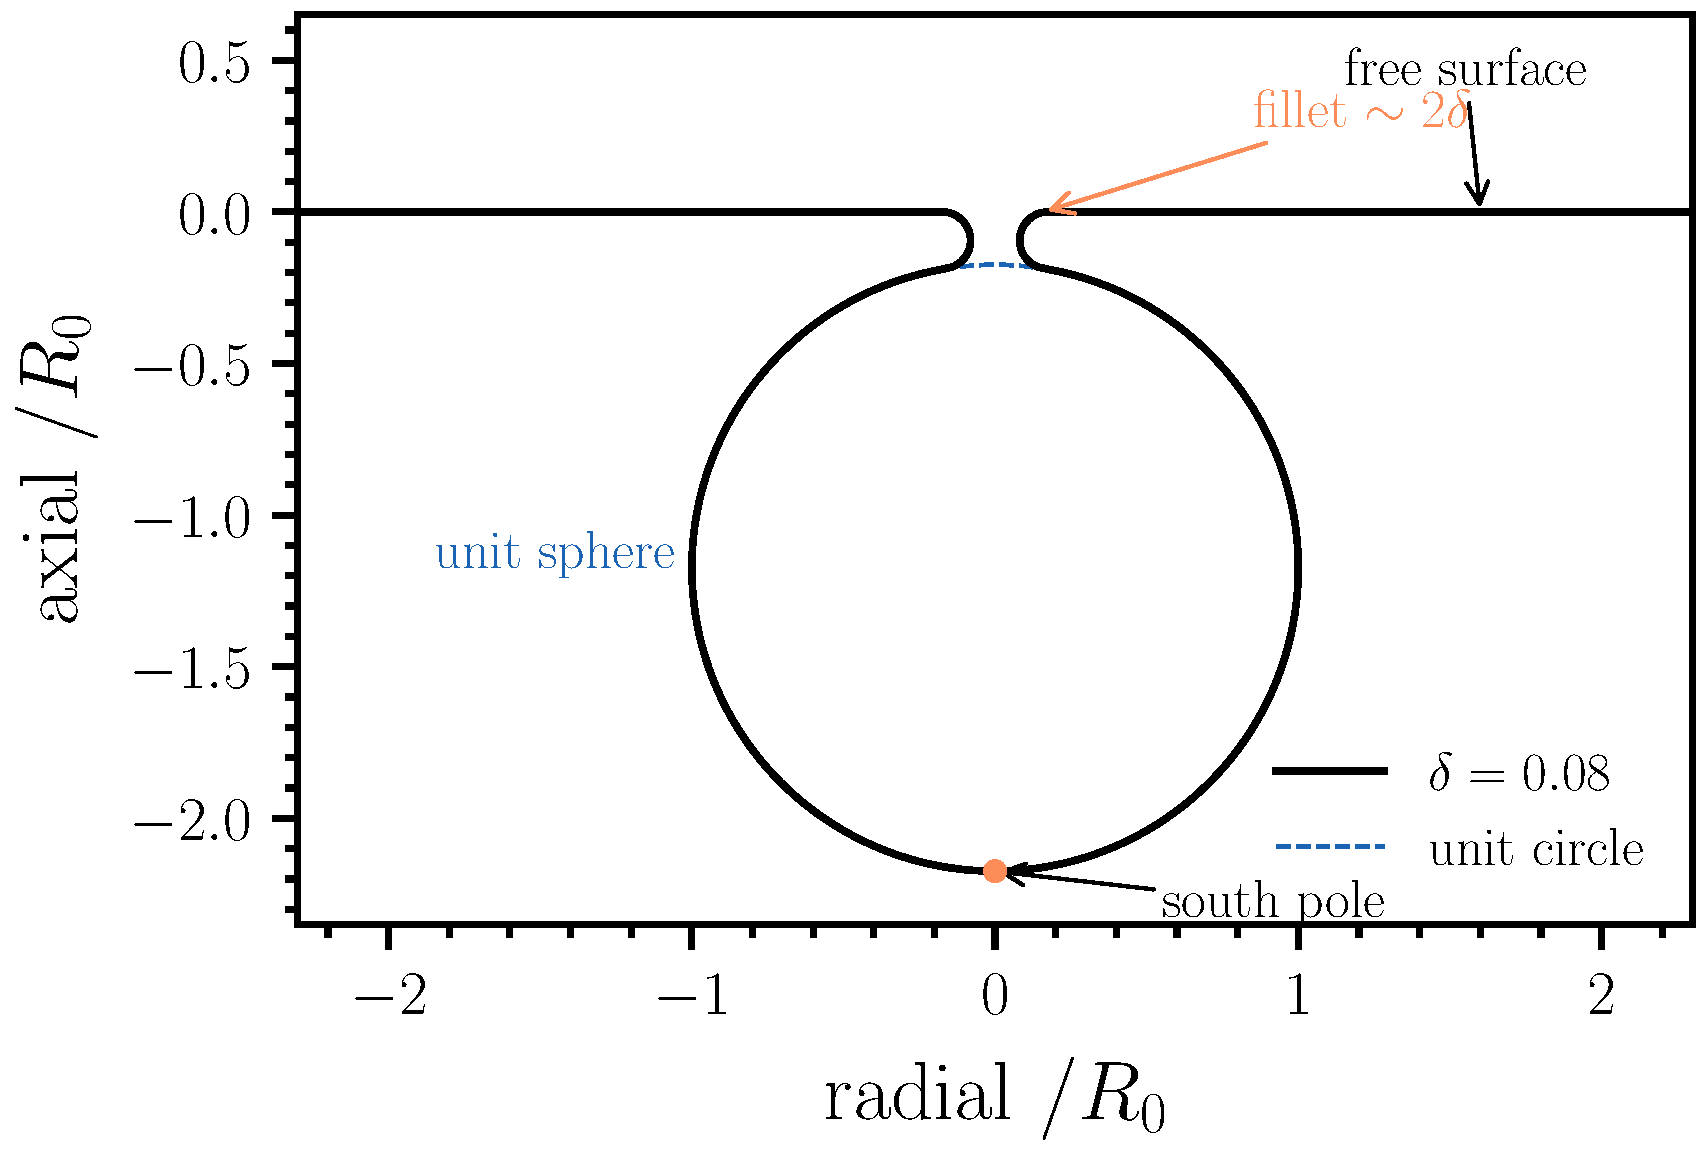
\includegraphics[width=0.72\textwidth]{zero_bond.pdf}
  \caption{Regularized $\Bo=0$ geometry.
    A unit sphere meets a plane. The fillet of scale $\delta$ opens a
    neck of radius $\sim 2\delta$ and replaces the point contact.
    The schematic uses $\delta=0.08$ so the neck is visible. The
    generator default is $\delta=0.01$.
    Coordinates are the Basilisk convention of \S\ref{sec:checks}.}
  \label{fig:zero}
\end{figure}

\section{File convention and checks}
\label{sec:checks}

Basilisk Stage~1 reads
\begin{center}
  \texttt{simulationCases/DataFiles/Bo\%5.4f.dat}
\end{center}
through \texttt{distance.h} and \texttt{input\_xy}. Column~1 is axial.
Column~2 is radial. The cavity lies in $-\mathrm{axial}$. The far-field
free surface sits at $\mathrm{axial}=0$. The south pole is the first
sample. \texttt{distance.h} is MPI-incompatible, so Stage~1 must
convert this polyline to a restart dump in serial (or OpenMP). Stage~2
then reads that dump and may run under MPI.

The repository ships \texttt{Bo0.0010.dat} as the current default
Stage~1 cavity. The geometry tests in \path{test_shapes.py} regenerate
that Bond number from a cold start and require the south pole to lie
within $0.01\,\Rzero$ of the shipped file, a volume residual below
$10^{-6}$, and the small-Bond opening \eqref{eq:alpha} to better than
eight percent. A cold start at $\Bo=1$ walks the continuation ladder
and does not return to the axis after leaving the south pole.

Figure~\ref{fig:opening} rebuilds the historical comparison.
The abscissa is $(\Rc/\Rzero)\sqrt{\Bo}=\Rc/a$. The ordinate is
$2\alpha_c/\pi$. The present generator tracks the digitised points of
\citet{Lhuissier2012} from $\Bo=10^{-4}$ to $\Bo=900$, including the
small-Bond line \eqref{eq:alpha} and the large-Bond saturation
$2\alpha_c/\pi\to 1$. That comparison is a literature check of the
shooter. It is not a claim about any particular bursting campaign.

\begin{figure}
  \centering
  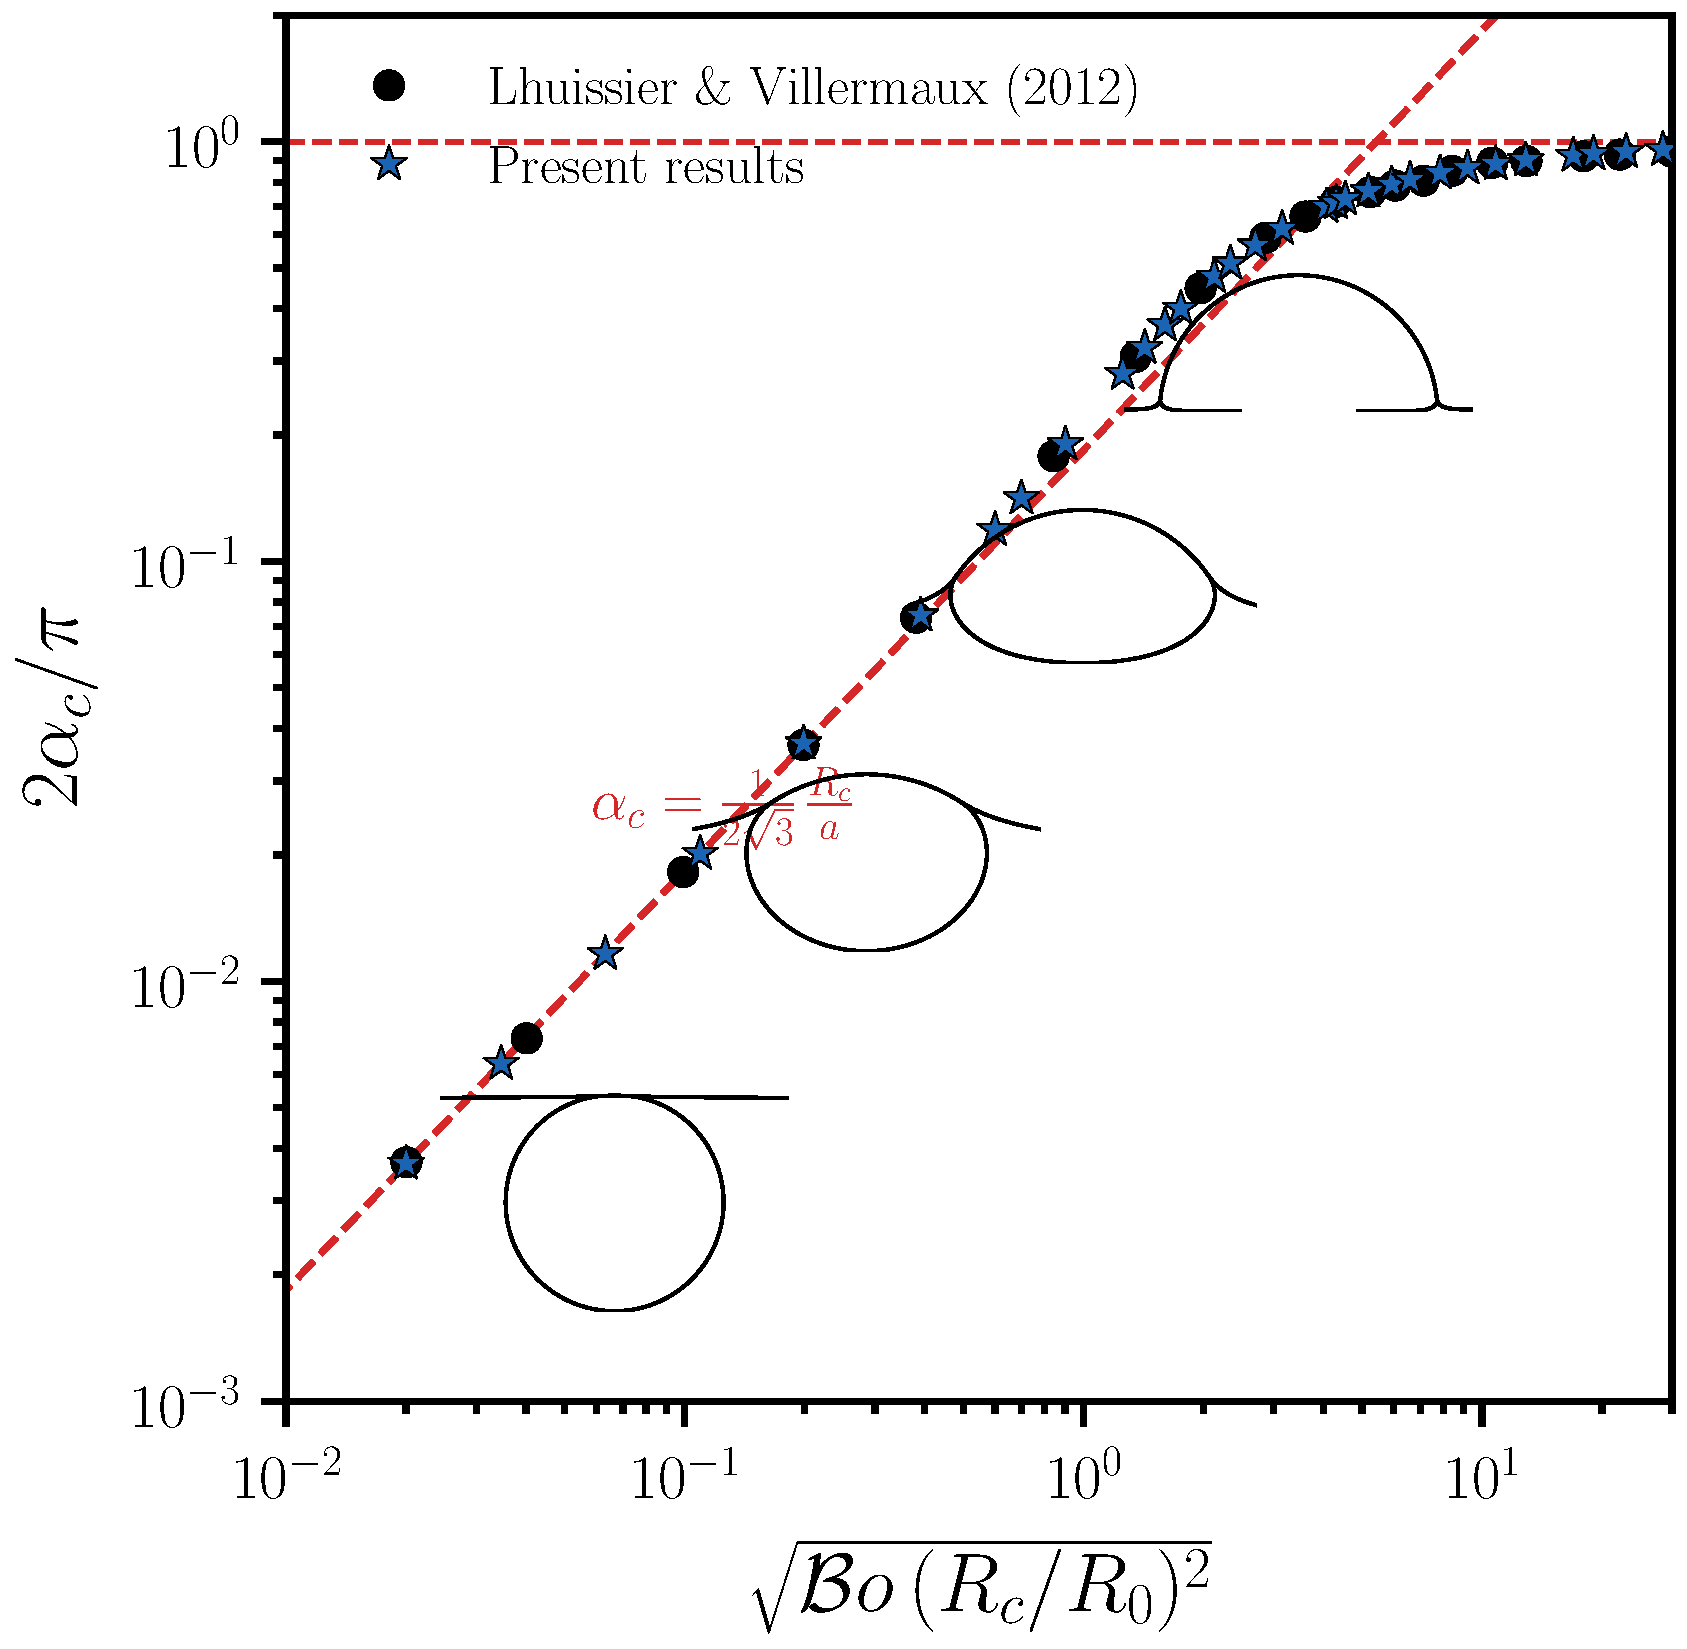
\includegraphics[width=0.78\textwidth]{opening_angle.pdf}
  \caption{Opening angle against the capillary length.
    Filled circles are the digitised data of \citet{Lhuissier2012}.
    Stars are the present continuation.
    The dashed line at small $\Rc/a$ is \eqref{eq:alpha}.
    The upper dashed line is $2\alpha_c/\pi=1$.
    Insets show the equilibrium cavity at selected Bond numbers.}
  \label{fig:opening}
\end{figure}

\section{Generating shapes}
\label{sec:cli}

The finite-Bond driver is \path{generate_bond_shape.py}.
The Bond-zero driver is \path{generate_zero_bond.py}.
Both write the Stage~1 convention of \S\ref{sec:checks}.

\begin{verbatim}
./.venv/bin/python generate_bond_shape.py --bond 0.001
./.venv/bin/python generate_bond_shape.py \
    --bond 0.01,1,10 --out-dir ../DataFiles
./.venv/bin/python generate_zero_bond.py --delta 0.01 \
    --out ../DataFiles/Bo0.0000.dat
\end{verbatim}

Pass \texttt{--no-continue} to force a one-shot solve at every Bond in
a list. That flag is a robustness check. It is not the recommended
path at large Bond. Geometry tests live in \texttt{test\_shapes.py}.
The opening-angle figure is rebuilt by
\texttt{plot\_opening\_angle.py}.

\section{Concluding remarks}
\label{sec:close}

The initial cavity of a bursting-bubble computation is a Young--Laplace
problem, not a sphere with a hole cut in it. Once Bond is finite the
nested shoot on $\Rb$ and $\varphi_c$, continued from a spherical seed,
gives a polyline that Stage~1 can ingest and that recovers the opening
angle of \citet{Lhuissier2012}. At vanishing Bond the same file
convention is filled by a regularized sphere--plane geometry.

We caution that this is a quasi-static construction after the film has
gone. The true shape of a bubble that has risen to a free surface
depends on how it got there, and on the rheology of the pool
\citep{Sanjay2021}. The fillet regularizes a singularity. It does not
restore the missing film. Those caveats belong to the bursting
calculation that consumes the file, not to the equilibrium generator.

\bibliographystyle{plainnat}
\bibliography{references}

\end{document}
